\section{Variational circuits applied to deep reinforcement learning}
Variational circuit or \textit{parametrised circuit}, are a type of quantum computing model that can be used in the field of machine learning. The problems that this model tries to tackle are: find the best parameters to solve the problem required and applicability to actual physical quantum devices with their limitations. This kind of circuit is \textit{hybrid}, because it uses concept that comes from quantum and classical algorithms, futhermore it can be applied to actual quantum devices with classical computer. The usual approach for this kind of circuit is to use quantum algorithms as the machine learning model and apply the training on data using classical algorithms. In this thesis it will be used as a layer for \acrfull{nn}, due to the fact that these kinds of circuits can be even viewed as \textit{quantum neural networks} thanks to their approximation ability to functions and because deep learning models are particularly successfull in \acrfull{rl}. A consideration that needs to be done is the fact that an ideal variational circuit must be small as possible in order to make it work on a quantum device and reduce the possibility of information loss due to decoherence, this type of circuit is referred as \textbf{shallow circuit}. An extensive paper that describes these circuit is \cite{Cerezo_2021}.
\subsection{Variational Circuit}
Variational circuits have been fromulated by \cite{https://doi.org/10.48550/arxiv.1802.06002}-\cite{Benedetti_2019}, but the idea was introduced years before. This circuit are based from the fact that gate can have an associated a parameter, the parametrized and unparametrized gates that will be used in the circuit will form an \textbf{ansatz}.In order to optimize the parametrized circuit it is necessary to define a cost function $C(\theta)$ and find an optimizer algorithm able to find the set parameters for which this cost function is minimized. This optimizer usually is based on gradient methods to reach the set of parameters that minimize the cost function, fortunately the gradient of a variational circuit can be calculated quite easily using a method called \textbf{parameter shift} as it will be seen later.\\
Thanks to the proprierties of quantum mechanics the entire circuit can be considered as a single unitary gate of the form $U(x,\theta)$ due to their dependecies on the input data. Usually the internal structure of $U(x,\theta)$ consist on of an embedding block $S(x)$ and a parametrized one $W(\theta)$ in order to decompose $U(x,\theta) = S(x)W(\theta)$, these blocks can contains quantum fixed gates. Graphycally this can be seen as:\\
\begin{center}
	\begin{figure}[!h]
		\centering
		\begin{tikzpicture}
		\node{
		\begin{quantikz}
			& \gate[wires= 3, style={fill=red!70}]{S(x)} & \gate[wires = 3, style={fill=cyan}]{W(\theta)} & \qw \\
			& & & \qw \\
			& & & \qw \\
		\end{quantikz}
		};
		\end{tikzpicture}
	\caption{ususal decomposition of quantum circuit}
	\label{sw}
	\end{figure}
\end{center}
So in the end a variational circuit can be graphically summarized as follows:
\begin{center}
	\begin{figure}[!h]
	\begin{tikzpicture}
		%%nodes
		\node[draw] (qc){
		\begin{quantikz}
			\lstick{$\ket{0}$} & \gate[wires= 3, style={fill=green}]{U(x, \theta)} & 	\meter{} & \qw\rstick[wires=3]{$f_{\theta}(x)$} \\
			\lstick{$\ket{0}$}& & \meter{} & \qw \\
			\lstick{$\ket{0}$}& & \meter{} & \qw
		\end{quantikz}
		};
		\node[draw,fill=Goldenrod, right=20mm of qc] (cost) {$C(\theta)$: cost function};
		\node[draw,fill=purple!40, below left=30mm and 1 mm of cost] (opt) {Optimizer: $\arg \min_{\theta} C(\theta)$};
		\draw[-stealth, line width=0.6mm] (qc.east) -- (cost.west);
		\draw[-stealth, line width=0.6mm] (cost.south) |- (opt.east);
		\draw[line width=0.6mm] (opt.west) -- node [midway,above,align=center ] {updated parameters($\theta$)} (-4.5,-3.7);
		\draw[line width=0.6mm] (-4.47,-3.7) -- (-4.5,0);
		\draw[-stealth, line width=0.6mm] (-4.53,0) -- (-3.3,0);
	\end{tikzpicture}
	\caption{Schematic of a variational quantum algorithm} 
	\label{vqa graph}
	\end{figure}
\end{center}
Furthermore these variational circuits can be interpreted, with minor conceptual changes, to deterministic or probabilistics machine learning models and can be ingtegrated, as it will be seen in this thesis, as a component of neural networks.\\
\subsubsection{Deterministic quantum model}
\begin{mydef}
	Considering a data domain $X$, the quantum circuit $U(x, \theta)$ with $x \in X, \theta \in \mathbb{R}^n$ depends on input data and indicating $\mathcal{M}$ as an hermitian operator associated to a quantum observable. It is possible to denote $\ket{\psi{x,\theta}}$ as  $U(x,\theta)\ket{0}$ then it is possible to define the output of this variational circuit as:
	\begin{equation}\label{quantum deterministic}
		f_\theta(x) = \bra{\psi(x, \theta)} \mathcal{M}  \ket{\psi(x, \theta)} = \braket{\mathcal{M}}_{x,\theta}
	\end{equation}
\end{mydef}
This formula tells that even if quantum computing output is statistical, an average value based on the measurement applied can be extracted. For example if measurement is written in diagonal basis such as : $\mathcal{M} = \sum_i \mu_i \ket{\mu_i} \bra{\mu_i}$, then the output function will be of the form of:
\begin{equation*}
	f_\theta(x) = \sum_i \mu_i |\braket{\mu_i |\psi(x, \theta)}|^2 = \sum_i \mu_i p(\mu_i)
\end{equation*}
In case the measurement applied is based on the Z-gate($\mathcal{M} = Z$) which will be the one iused in the following variational quantum algorithm the result can be rewritten by considering the eigenvalues and eigenstates obtaining the following result:
\begin{equation*}
	f_\theta(x) = |\braket{0|\psi(x, \theta)}|^2 - |\braket{1| \psi(x, \theta)}|^2 = p(0) - p(1)
\end{equation*}
This quantity can be even calculated by performing $S$ shots sampling the eigenvalues $\mu^(s) \in {\mu_i}$ and averaging over the results, obtaining the following form:
\begin{equation*}
	\hat{f}(x) = \frac{\sum_{i=1}^{S}\mu_i}{S}
\end{equation*}
This value can be estimated with an error $\epsilon$ applying $O(\epsilon^{-2})$ measurement, this means that if for example the error required is 0.01, then the measurement needed to be applied is of the order in 1000s. This deterministic function will be used mainly for approximating the q-value and other quantity necessary for the reinforcement learning algorithm. 
\subsubsection{Probabilistic quantum model}
The inherit theory of quantum mechanics allows for these models to be expressed as probabilistic, in fact as it will be seen later \acrfull{vqa} can be interpreted as supervised and unsupervised model applying minimal modifications on the quantum circuit.
\begin{mydef}[supervised probabilistic quantum model]
	Let $X$ be an input and $Y$ an output domain, and $U(x, \theta)$ be an input and parameter-
	dependent unitary so that $\psi(x, \theta) = U(x, \theta)\ket{0}$. We associate each eigenvalue	or outcome of a measurement observable with a possible output $y$, so that $\mathcal{M} \sum_{y \in Y} y \ket{y} \bra{y}$. A supervised probabilistic quantum model for a conditional distribution is then defined:
	\begin{equation}
		p_\theta(y|x) = |\braket{y|\psi(x, \theta)}|^2
	\end{equation}
\end{mydef}
Due to ${\ket{y}}$ being a basis, the normalization is required so $\sum_{y \in Y} \ket{y} \bra{y} = \mathbbm{1}$ and probability sum to 1.Representing this kind of variational quantum circuit using the previous ansatz, it can be represented as:
\begin{center}
	\begin{figure}[!h]
		\centering
		\begin{tikzpicture}
			\node{
				\begin{quantikz}
					\lstick{$\ket{0}$} & \gate[wires= 3, style={fill=red!70}]{S(x)} & \gate[wires = 3, style={fill=cyan}]{W(\theta)} & \meter{} & \qw\rstick[wires=3]{$y \sim p_\theta (y|x)$} \\
					\lstick{$\ket{0}$}& & & \meter{} & \qw \\
					\lstick{$\ket{0}$}& & & \meter{} & \qw
				\end{quantikz}
			};
		\end{tikzpicture}
		\caption{Variational quantum algorithm for conditional probability}
		\label{vqa conditional}
	\end{figure}
\end{center}
This kind of circuit has been used for classification and regression tasks mainly, but as it will be seen that can be used in reinforcement learning to decide which action to take in a discrete environment.\\
\begin{mydef}[unsupervised probabilistic quantum model]
	Let $X$ be an input	domain, $W(\theta)$ a unitary that depends on some parameters with $\ket{\psi(\theta)} = W(\theta) \ket{0}$, and $\mathcal{M} = \sum_{x \in X} x \ket{x} \bra{x}$a measurement in diagonal basis with outcomes that correspond to the inputs $x$. An unsupervised probabilistic quantum model is defined by the distribution:
	\begin{equation}
		p_\theta(x) = |\braket{x|\psi(\theta)}|^2
	\end{equation}
\end{mydef}
The circuit can be graphically defined as:
\begin{center}
	\begin{figure}[!h]
		\centering
		\begin{tikzpicture}
			\node{
				\begin{quantikz}
					\lstick{$\ket{0}$} & \gate[wires = 3, style={fill=cyan}]{W(\theta)} & \meter{} & \qw\rstick[wires=3]{$x \sim p_\theta (x)$} \\
					\lstick{$\ket{0}$} & & \meter{} & \qw \\
					\lstick{$\ket{0}$} & & \meter{} & \qw
				\end{quantikz}
			};
		\end{tikzpicture}
		\caption{Variational quantum algorithm for unsupervised approach}
		\label{vqa unsupervised}
	\end{figure}
\end{center}
So it is possible to notice that the only differences between the unsupervised and supervised model are two: the absence of embedding layer and data basis for measurement instead of the output basis.Probabilistic quantum model is strictly correlated to deteminsitc one due to the fact that $p_\theta(x) = |\braket{x|\psi(\theta)}|^2$ can be even seen as $\bra{x}(\ket{\psi(\theta)} \bra{\psi(\theta)}) \ket{x}$ with basis measurement of $\mathcal{M} = \ket{\psi(\theta)} \bra{\psi(\theta)}$. This is important because it define a clear connection betwenn the insights on designs applied. Futhermore it is possible to notice that \acrshort{vqa} are generative models, but it is difficult to extract this distribution due to the measurements requried. Lastly unsupervised quantum models are even known as \textit{Born machines} from the Born rule that links quantum states and probability.
\subsubsection{Quantum models as linear combinations of periodic functions}
For generality it is possible to express the quantum circuit using in the model as an alternation between encoding an parametrized gates repeated for multiple layers as:
\begin{equation}\label{udecomp}
	U(x,\theta) = W_{N+1}(\theta) = \prod_{i = 1}^{N} S_i(x_i)W_i(\theta)
\end{equation}
embedding gate can be defined as having the form $S_i(x_i) = e^{-i x_i G_i} $ where $G_i$ without losing genrality can be assumed a diagonal operator $diag(\lambda_{i}^{1}, \dots, \lambda_{i}^{1} )$ with d dimension of Hilbert space. Then a theorem proven by \cite{Schuld_theorem} demonstrate the linear combination of such models.
\begin{theorem}
	Let $X \in \mathbb{R}^n$, $Y = \mathbb{R}$ and $f_\theta:X \to Y$ be a deterministic quantum model with a circuit $U(x,\theta)$ as defined in \ref{udecomp}. Accordingly the i-th  feature is encoded by gate $ e^{-i x_i G_i}$: Then $f_\theta$ can be written as 
	\begin{equation*}
		f_\theta(x) = \sum_{w_1 \in \Gamma_1} \dots \sum_{w_N \in \Gamma_N} c_{w_1 \dots w_n}(\theta) e^{iw_1 x_1} \dots e^{iw_N x_N}
	\end{equation*}
	with the frequency spectrum of the i-th feature, $i=1,\dots,N$ is given by 
	\begin{equation*}
		\Gamma_i = \{\lambda_{s}^{i} - \lambda_{t}^{i} | s, t \in {1, \dots,d} \}
	\end{equation*}
	This frequency spectrum is the set of all values produced by differences between
	any two eigenvalues of $G_i$ . We are guaranteed that $0\in\Gamma$, and for each $w \in \Gamma$	there is $-w \in \Gamma$ too with $c_w(\theta) = c_{-w}^{*}(\theta)$. This symmetry guarantees that $f_\theta$ is real-valued, and that the sum can be rewritten with cosine and sine functions.
\end{theorem}
This theorem is important because it tells that there is no linearity if only the variational cirucit is applied, the frequencies are defined by the embedding layer and weights are dependent on parameters and frequencies. This means that for an expressive \acrlong{vqa} the embedding and parameters layer must be repeated multiple times to have enough expressitivity.
This means that unfortunately non-linearity is not present on these circuits, unless measurement or specific gate are introduced as it will be seen later.
\subsubsection{Variational algorithm training}
As previously stated this type of cicruit is parametrized and the parameters are optimized by calculating a cost function and the gradient. Due to the fact that cost fucntion is dependendant in first place from output function and afterward to parameters, the chain rule needs to be applied obtaining the following equation:
\begin{equation}
	\frac{\partial C(\theta)}{\partial \mu} = \frac{\partial C(\theta)}{\partial f(\theta)} \frac{\partial f(\theta)}{\partial \mu} 
\end{equation}
This form has two components $\frac{\partial C(\theta)}{\partial f(\theta)}$ and $\frac{\partial f(\theta)}{\partial \mu}$ required to exactly calculate the differentiation. First one can be obtained using classical computation, while the second one cannot be evaluated using classical quantities because it depend directly on the quantum circuit.
In fact using the parameter-shift rules it possible to calculate the gradient of a quantum circuit compared to the parameters $\frac{\partial f(\theta)}{\partial \mu}$ , while for the other quantity library such as \textit{Tensorflow} and \textit{Pytorch} can apply \textbf{automatic differentiation} to approxiamte the result.\\
\begin{mydef}[parameter-shift rules]
Let $f_\mu = \braket{\mathcal{M}}_\mu$ be a quantum expectation value that depends on a classical parameter $\mu$. A parameter-shift rule is an identity of the form:
\begin{equation}
	\partial_\mu f_\mu = \sum_{i} a_i f_{\mu + s_i}
\end{equation}
where ${a_i}$ and ${s_i}$ are real scalar value.
\end{mydef}
As it can be noticed this formula is similar to the finite difference method which is:
\begin{equation*}
	\frac{\partial f_\theta}{\partial \mu} \approx \frac{f_\theta - f_{\theta + \Delta \theta}}{||\Delta \theta||}
\end{equation*}
the main difference is that \textbf{the parameter-shift rule method is able to estimate the analytic gradient, while the finite difference method focus on approximating it}. Furthermore the parameter-shift rule is not dependant on how big or small must be the variation in order to correctly calculate the gradient and requires very few evaluations.
There is a problem with the gradients of variational circuits, that is a significant presence of \textbf{barren plateaus}. This term refers to the fact that sometimes the cost function can presents zone where the gradient is highly probable to be zero leading to small variantons on gradient. Mathematically speaking this means that:
\begin{equation}\label{barren plateau}
	Var[\partial_\mu f_\mu] = 0
\end{equation} 
This is a problem for the correct optimization of parameters due to the fact that gradient is particularly small leading to a non global minimal solution or requiring a great amount of training time before actually leaving this zone. The \textbf{barren plateaus} are present in \acrlong{nn} and is something studied and discussed, but no real solution has been actually found to deal with it.
Difference between classical and quantum model is the fact that these regions are \textbf{\textit{exponentially more large}} on the quantum case as demonstrated by \cite{McClean_2018}. The paper furthermore explains that increasing the number of gates, referred even as layers due to repetition of specific gates, and qubits leads to an exponential decay on the variance. This is an ulterior motive for which the variational circuit that is defined must be the most shallow in order to avoid problems on trainability. There has been some strategy addressed to partially solve this problem such as initialization using correlated parametrized circuit as suggested by \cite{Grant_2019}, but this represent one of the major challenge to solve in order to use deepest circuits. A deeper and more detailed explaination can be found in \cite{Schuld2021vqa}.
\subsubsection{Variational algorithm as neural networks}
Variational circuits are sometimes called "quantum neural networks". This name is partially reasonable due some resemblance to classical neural network such as the optimization of parameters and structure linearity for deep learning. Problem is that these circuits does not express non-linearity unless particularly encoding strategy or measurement is applied. 
In a interesting wa, non-linear activation function can be obtained by applying different types of encoding with slight modifications as suggested by \cite{Schuld2021vqa}, but the papers to create the ansatz for reinforcement learning does not apply them. It would be intersting to see if these encoding may result in a better performance on future tests.
A possible schematic on how \acrlong{vqa} can be interpreted as \acrlong{nn} is given by figure \ref{vqa nn}.From this schematic it can be observed an important fact the only non-linearity present is due to the measurement applied at the end. To introduce more non-linearity gates such as \textit{depolarizing gates} and even \textit{noise} can be added, but this is not a complete solution. Furthermore it can be noticed how every gate applied can be associated to a layer o f the neural network.
Possible representation that can be used is to define a formalism linked to connectivity by generalizing a single qubit gate as:
\begin{equation*}
	W = \begin{bmatrix}
		z & u \\
		-u* & z*
	\end{bmatrix}
\end{equation*}
\begin{center}
	\begin{figure}[!h]
		\centering
		\begin{tikzpicture}
			\node[circle, fill=red!70, label={input}] (I-1) at (-0.2,-1) {};
			\node[circle, fill=cyan, label={linear}] (H-1) at (1.7cm,-1 cm) {};
			\node[circle, fill=cyan, label={linear}] (H_-1) at (3.4cm,-1 cm) {};
			\node[circle, fill=lime, label={non-linear}] (O-1) at (5.2cm,-1 cm) {};
			% Draw the input layer nodes
			\foreach \y in {2,...,4}{
				% This is the same as writing \foreach \name / \y in {1/1,2/2,3/3,4/4}
				\node[circle, fill=red!70] (I-\y) at (-0.2,-\y) {};
				\node[circle, fill=cyan] (H-\y) at (1.7cm,-\y cm) {};
				\node[circle, fill=cyan] (H_-\y) at (3.4cm,-\y cm) {};
				\node[circle, fill=lime] (O-\y) at (5.2cm,-\y cm) {};
			}
			\foreach \n in {1,..., 4}{
				\foreach \m in {1,..., 4}{
					\path (I-\n) edge (H-\m);
					\path (H-\n) edge (H_-\m);
					\path (H_-\n) edge (O-\m);
				}
			}
						
			\node[below = 10 mm of H-4](vc) {
				\begin{quantikz}
					\lstick{$\ket{0}$} & \gate[wires= 3, style={fill=red!70}]{S(x)} & \gate[wires = 3, style={fill=cyan}]{W_1(\theta)}& \gate[wires = 2, style={fill=cyan}]{W_2(\theta)} & \meter[style={fill=lime}]{}  \\
					\lstick{$\ket{0}$}& & & & \meter[style={fill=lime}]{} \\
					\lstick{$\ket{0}$}& & & \gate[style={fill=cyan}]{W_3(\theta)} & \meter[style={fill=lime}]{}
				\end{quantikz}
			};
		\end{tikzpicture}
		\caption{Variational quantum algorithm as a neural network}
		\label{vqa nn}
	\end{figure}
\end{center}
This matrix representation must respect the condition of normalization. In case the single qubit gate is applied on only one qubit, for example $i$, a multi-qubit representation can be defined by extending the previous definition:
\begin{equation*}
	W_i = \mathbbm{1} \otimes \dots \otimes \underbrace{W}_{i\;position} \otimes \dots \otimes \mathbbm{1}
\end{equation*}
The simbol $\mathbbm{1}$ refers to an identity matrix $2\times2$, this means that a single qubit gate applied leads to a sparse representation and the matrix able to represent any kind of operation applied on multiple qubits has shape $2^n \times 2^n$. This is interesting and gives a connection between layer of neural network with linear activation and vqa because both of them use matrix operations.
\subsubsection{Data reuploading}
As it was already explained before, the \acrlong{vqa} are linear except for the final points where measurement is applied. This can be problematic for the field of deep reinforcement due to significant presence of non-linear functions for the q-values and actor component. In order to introduce this non-linearity and deal with the \textbf{non-cloning} property of quantum computing a new type of ansatz has been defined: \textit{\textbf{data reuploading}}.
This concept has been introduced in the paper \cite{P_rez_Salinas_2020} and it wants to introduce non-linearity by reapplying the embedding layer multiple times in order to have a more composite function expressivity. So the strategy is to not use more qubits, but apply multiple layer increasing the depth of final circuit. This seems to work particularly well for reinforcement learning using simulators. Question is if this kind of depth would be able to run omn a quantum computer and will be a ble to achieve the same performance. This is something that may be required further work.
\subsection{Quantum Deep Q-learning applied to Cartpole} 
Now that \acrlong{vqa} has been explained it is now time to see the results obtained by applying qauntum models on the environment called Cartpole-v0. This is part of the library Open-AI gym (\cite{1606.01540}, \href{https://www.gymlibrary.ml/}{link}), which contains multiple environments used for benchmarking reinforcement learning algorithms.\\
The Cartpole environment is composed by a pole attached to a cart:
\begin{figure}[h]
	\centering
	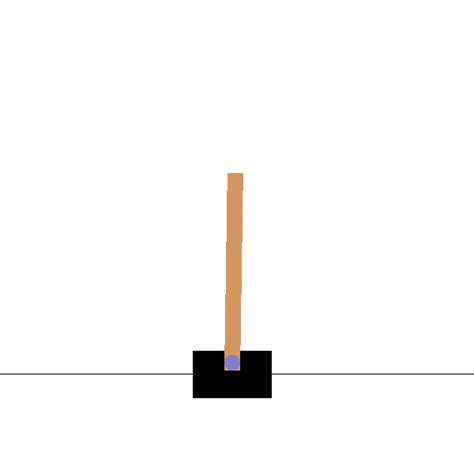
\includegraphics[width=0.7\linewidth]{img/cartpole}
	\caption[Cartpole environment]{Cartpole environment of Open-AI gym}
	\label{fig:cartpole}
\end{figure}\\
The environment state is an array of 4 values representing: (position, velocity, pole angle, pole angular velocity). Position and angle are limited in value, while the others are not. The possible action that can be taken is a single value tha can be 0 or 1, which respectivelly means push left or right. The reward given by the environment is that for every step taken the total reward is increased by 1 even on termination. The conditions for which an episode is stopped are: the cartpole reaches extrems of the environment, angle pole is equal or greater than 12° or the number of steps taken is equal to 200.\\
The goal is to reach a reward greater or equal than 175 for 100 episodes. Technically when this condition is reached the training should be stopped, but it will be extended for 1000 episodes in order to check the stability and convergence of the algorithm. To confront the advantage between \acrlong{nn} and \acrlong{vqa} it will be counted the trend of reward, the number of episode taken to reach the goal, time taken and numbers of parameters.
This has been decided from reference of other papers that used this way to benchmark classical and quantum models.\\
\subsubsection{Ansatz for VQA}
Different ansatz have been used for this work, the starting point was form the paper \cite{Scholik_2022} which has a corresponfing github repository that can be used for the code.
Variational circuit proposed for the paper is based from the following layer:
\begin{figure}[!h]
	\centering
	\begin{tikzpicture}
			\node(vq) {
				\begin{quantikz}
					\qw & \gate[style={fill=red!70}]{R_x(x)} & 	\gate[style={fill=cyan}]{R_y(\theta)}& \gate[style={fill=cyan}]{R_z(\theta)} & \ctrl{1} & \qw & \qw & \targ{} & \qw  \\
					\qw & \gate[style={fill=red!70}]{R_x(x)} & 	\gate[style={fill=cyan}]{R_y(\theta)}& \gate[style={fill=cyan}]{R_z(\theta)} & \targ{} & \ctrl{1} & \qw & \qw & \qw \\
					\qw & \gate[style={fill=red!70}]{R_x(x)} & 	\gate[style={fill=cyan}]{R_y(\theta)}& \gate[style={fill=cyan}]{R_z(\theta)} & \qw & \targ{} & \ctrl{1} & \qw & \qw \\
					\qw & \gate[style={fill=red!70}]{R_x(x)} & 	\gate[style={fill=cyan}]{R_y(\theta)}& \gate[style={fill=cyan}]{R_z(\theta)} & \qw & \qw & \targ{} & \ctrl{-3}  & \qw
				\end{quantikz}
			};
		\end{tikzpicture}
	\caption{Variational quantum algorithm for cartpole }
	\label{vqa dqn}
\end{figure}\\
As it can be seen, this kind of layer applies the data-reuploading approach already mentioned. This seems vital in order to achieve a good performance in respect to the classical one, for more detail please consult the paper. This kind of layer is repeated multiple times in order to achieve enough depth for the expresssivity required to approximate the best q-value function. The measurement applied at the end uses probabilistic approach, in fact due to the nature of cartpole a single action is required, go left or right, so in order to reduce the dimension output a measurement composed on two qubits corresponding to $Z \otimes Z$ is applied. After the measurement value with maximum probability is chosen and executed. In order to increase the performance a classical layer of weights on input and output is added, this leads to the folloring final structure.
\begin{figure}[!h]
	\centering
	\resizebox {1.1\linewidth} {!} {
	\begin{tikzpicture}
		\node[draw, label = {repeat $n$ times}](dqn) {
			\begin{quantikz}
				\qw & \gate[style={fill=red!70}]{R_x(x)} & 	\gate[style={fill=cyan}]{R_y(\theta)}& \gate[style={fill=cyan}]{R_z(\theta)} & \ctrl{1} & \qw & \qw & \targ{} & \qw   \\
				\qw & \gate[style={fill=red!70}]{R_x(x)} & 	\gate[style={fill=cyan}]{R_y(\theta)}& \gate[style={fill=cyan}]{R_z(\theta)} & \targ{} & \ctrl{1} & \qw & \qw & \qw \\
				\qw & \gate[style={fill=red!70}]{R_x(x)} & 	\gate[style={fill=cyan}]{R_y(\theta)}& \gate[style={fill=cyan}]{R_z(\theta)} & \qw & \targ{} & \ctrl{1} & \qw & \qw  \\
				\qw & \gate[style={fill=red!70}]{R_x(x)} & 	\gate[style={fill=cyan}]{R_y(\theta)}& \gate[style={fill=cyan}]{R_z(\theta)} & \qw & \qw & \targ{} & \ctrl{-3} & \qw
			\end{quantikz}
		};
		\node[right= -4mm of dqn, label = {measure}](measure) {
			\begin{quantikz}
				\qw & \gate[wires =2]{Z \otimes Z} \\
				\qw & \qw \\
				\qw & \gate[wires =2]{Z \otimes Z}\\
				\qw & \qw 
			\end{quantikz}
		};
		\node[circle, above left = -8mm and 10mm of dqn , fill=orange, label={input}] (I1) {};
		\node[circle, below = 8mm of I1 , fill=orange] (I2) {};
		\node[circle, below = 8mm of I2 , fill=orange] (I3) {};
		\node[circle, below = 8mm of I3 , fill=orange] (I4) {};
		\path (I1) edge (-4.95,1.8);
		\path (I2) edge (-4.95,0.6);
		\path (I3) edge (-4.95,-0.60);
		\path (I4) edge (-4.95,-1.8);
		\node[circle, above right = -15mm and 25mm of dqn , fill=orange, label={output}] (O1) {};
		\node[circle, below = 18mm of O1 , fill=orange] (O2) {};
		\path (6.9, 1.1) edge (O1);
		\path (6.9, -1.1) edge (O2);
	\end{tikzpicture}
}
	\caption{Final structure for cartpole}
	\label{dqn hybrid}
\end{figure}
The original implementation used as libraries pennylane and pytorch, this made the algorithm take around 11 hours for 5000 episodes. Due to the requirement of benchmarking the code has been rewritten using tensorflow quantum. This allowed a speedup by reducing the time required ...\\
By applying multiple runs and confronting the runs made by the quantum algorithm and different kind of neural network this result is obtained:
\begin{figure}[!h]
	\centering
	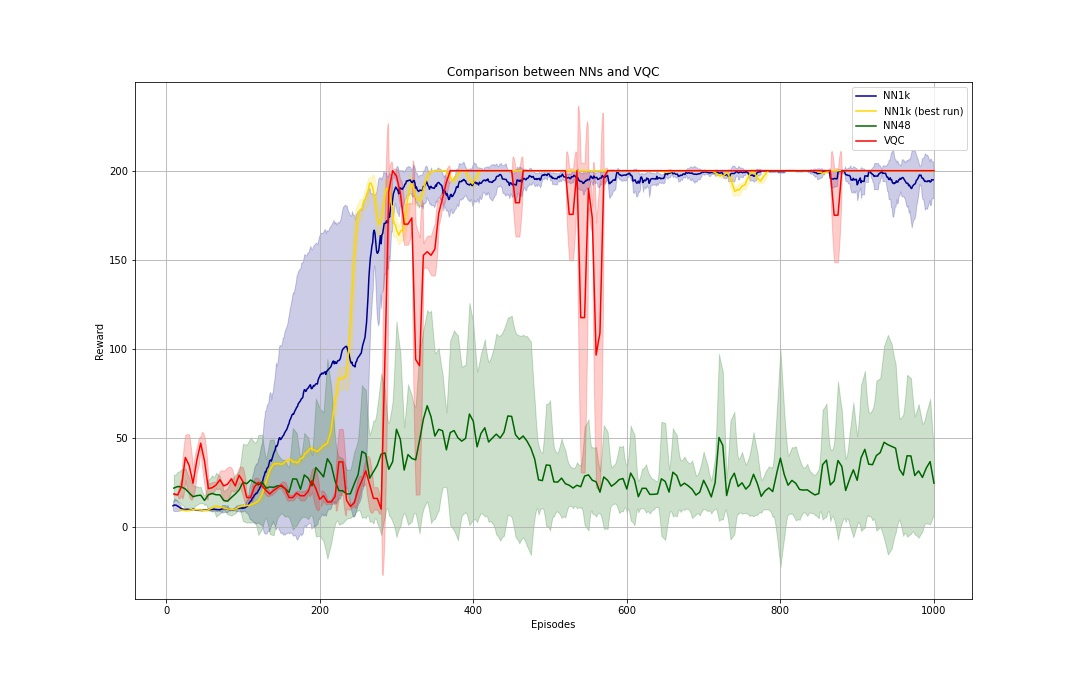
\includegraphics[width=\linewidth]{img/VQCNNcomparisonmedia}
	\caption[Benchmark of quantum and classical dqn]{In this image it has been used the mean and the variance of 10 runs of neural networks and vqa}
	\label{fig:vqcnncomparisonmedia}
\end{figure}\\
As it can be seen from the figure a neural network with the same number of vqa parameter is unable to reach the goal of cartpole and in order to have the same trend a neural network with 1256 parameters.\\
This means that a quantum advantage on the number of parameters and expressivity of the modes with few layers. The paper referenced is more expressive and even more detailed on all hyperparameters that has been tested, the configuration used for this benchmark is:
\begin{center}
	\begin{tabular}{|c|c|c|c|}
		\hline
		hyperparameter & NN(1256 params) & NN(48 params) & VQA \\
		\hline
		$\gamma$ & 0.99 & 0.99 & 0.99 \\
		\hline
		optimizer & Adam & Adam & Adam \\
		\hline
		batch size & 64 & 64  & 16 \\
		\hline
		learning rate & 0.001 & 0.001 & 0.01 \\
		\hline
		buffer memory & 100000 & 100000 & 10000 \\
		\hline
		$\epsilon$ start & 0.1 & 0.1 & 1 \\
		\hline
		$\epsilon$ decay & 0.99 & 0.99 & 0.99 \\
		\hline
		$\epsilon$ final & 0.001 & 0.001 & 0.01 \\
		\hline
		Loss & Smooth-L1 & Smooth-L1 & Smooth-L1 \\
		\hline
		neuron layers & (4,32)(32,32)(32,2) & (4,8)(8,2) & (4,)(2,)  \\
		\hline
		vqa layers & None & None & 5 \\
		\hline
	\end{tabular}
\end{center}
As it can be seen from the hyperpaprameters $\epsilon$ used for the $\epsilon$-greedy algorithm used is decreased from starting to ending value applying a formula called linear decay.\\
A better and more efficient ansatz was proposed by tensorflow quantum exactly for this kind of problem giving to the following structure of the \acrlong{vqa}:
\begin{figure}[h]
	\centering
	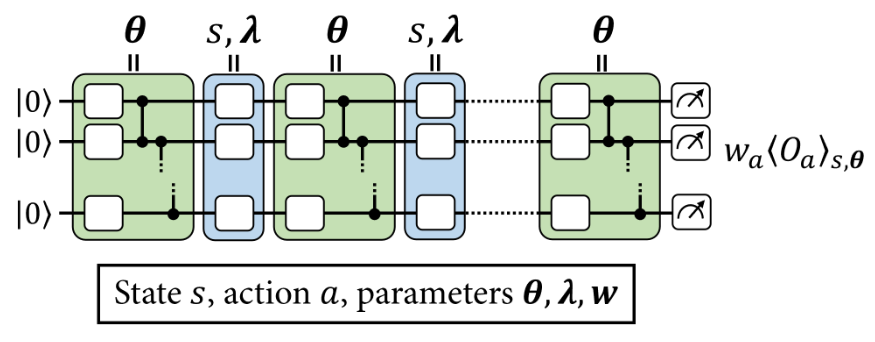
\includegraphics[width=0.8\linewidth]{img/tfq}
	\caption{Ansatz of variational circuit with data reuploading of the tensorflow quantum library}
	\label{fig:tfq}
\end{figure}\\
The differences between this kind of ansatz and \ref{dqn hybrid} are: the lack of classical weights input-output and most importantly the encoding layer is parametrized. This means that the expressivity of this model can be tuned by finding the parameters that are able to give the best encoding to find afterward best approximation.
%%%%%%%%%%%%%%%%%%%%%%%%%%%%%%%Important
%%from here i need my results
Now that the results of Cartpole has been showed proving that there can be a qantum advantage using less parameters, it is now change for another environment which is based on the robotic arm and can be a demonstration on the quantum capabilities applied on possible future industrial application.
\subsection{Variational quantum algorithm on robotic arm}
\subsubsection{Environment}
The previous environment is used for benchmarking and to have a partial view on the capability of this algorithm. It is now time to test it on something more difficult and with application on the industry: a robotic arm. This technology is applied in many field of industry such as: manufacturing, cars and many others.The environment that will be used to simulate a robotic arm has been created and offered from prof.Noah Klarmann from the university of Rosenheim who I would like to thank.This environment is formed of an arm composed of different links whose number can be defined, this influence both the space of state and action, with a randomic point which need to be reached by the arm using his extremis. The links are independent and can move on any direction with a fixed maximum velocity, this means that for every possible point that can be reached the number of steps required is not always the same.As it can be seen from this rendering:
\begin{figure}[h]
	\centering
	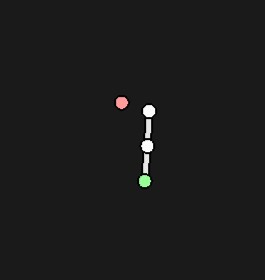
\includegraphics[width=0.45\linewidth]{img/quantum_robotic_arm_SAC_4182}
	\caption{Robotic arm with 2 links, the termination point of arm is green and the objective point is red}
	\label{fig:roboticarmsac}
\end{figure}\\
The total return is calculated every step taken, the value is negative for every step that the arm was unable to reach the determined point and is defined as the eukledian distance between arm termination and point. In case the arm is able to effectively reach the point a positive reward of +5 is given and the episode is considered ended. The termination conditions are two: the steps taken is equal to 250 or the point is reached. The state tuple is composed in case of 2 links: (target x, targe y, end effector x, end effector y, link angle 1, link angle 2) in case of more link the tuple increase considerinfg more angles. The action tuple has length equal to links and for the case of 2, it is : (link 1 velocity, link 2 velocity).There isn't an exact condition for which the environment is considered solved, but from multiple runs and afterward rendering the environment was decided to be considered solved when the mean reward was above 40 for the case of 2 links.
Differerently from the cartpole enviornment, robotic arm can be multidiscrete or continous and for application it was decided to use the continuos one and use the \acrfull{sac} by substituting a complete neural network approach with an hybrid which uses the \acrshort{vqa}.
\subsubsection{Quantum SAC}
A paper has been already published which uses a quantum \acrshort{sac} approach to solve the pendulum-v0 environment, the details can be found in \cite{https://doi.org/10.48550/arxiv.2112.11921}.
\begin{algorithm} \label{qsac}
	\caption{Variational Quantum Sac}
	\begin{algorithmic}
		\REQUIRE initial policy parameters $\theta$, initial action-value estimate parameters $\phi_1$ and $phi_2$, $\gamma$, $\alpha$, $\rho$, empty experience replay $D$.
		\STATE Initialize the hybrid quantum-classical policy network with $\theta$.
		\STATE Initialzie two action value networks with $\phi_1$ and $phi_2$ respectively.
		\STATE Set target-action value networks parameters: $\phi_{targ, 1} \leftarrow \phi_1$ and $\phi_{targ, 2} \leftarrow \phi_1$.
		\FOR{each time-step}
			\STATE Observe state $S$, select action $A \sim \pi_{\theta}(\cdot |S)$ and execute $A$ in the environment.
			\STATE Observe next state $S'$, reward $R$, and binary done signal $d$ to indicate whether $S'$ is terminal state or not.
			\STATE Store $(S,A,R,S',d)$ in $D$.
			\STATE Reset the environment if $d=1$.
			\STATE Sample a batch of transitions $B = {(S,A,R,S',d)}$ from $D$ randomly.
			\STATE Compute target values $y(R,S',d) = R + \gamma (1-d) (min_{i=1,2}Q_{\phi_{targ,i}} (S',A') - \alpha \log \pi_{\theta}(A',S'))$ where $A' \sim \pi(\cdot,S')$.
			\STATE Update $\phi_i$ by minimizing: $\mathbb{E}_B [(Q_{\phi_i}(S,A) - y(R,S',d))^2]$ for $i = 1,2$.
			\STATE Update $\theta$ by maximizing: $\mathbb{E}_B [min_{i=1,2} Q_{\phi_i}(S,\tilde{A}_\theta) - \alpha \log \pi_{\theta}(\tilde{A}_\theta|S)]$.
			\STATE Do a soft update for target action-value networks: $\phi_{targ,i} \leftarrow \rho \phi_{targ,i} + (1-\rho)\phi_i$ for $i=1,2$.
		\ENDFOR
	\end{algorithmic}
\end{algorithm}\\
So from this algorithm it is possible to understand that there 5 components necessary: an actor policy, two action-value approximator and others two called target action-value approximator.
The reason for which it is necessary the target components is similar to the \acrshort{dqn} case, due to the fact that usually two consecutive states are not independent and requiring action-values to be it in order to correctly update the weights an independent copy is required.
The reason for which both of action and target components is double can be explained from other advances of \acrshort{dqn} which showed that using two components and taking minimum of the two improves performance and stability.
The final component which is an actor policy, for the case of \acrshort{sac} this component will output two values: mean and variance of a gaussian distribution. From this the action will be sampled randomically meaning that this approach is statistical, it can be converted to deterministic by using the mean extracted from the component.\\
This policy actor in the paper is defined as a quantum-classic hybrid approach that differently form \acrshort{dqn} tries to incorporate \acrlong{nn} layers and \acrlong{vqa}. An image showing the actual structure is present on the paper:
\begin{figure}[h]
	\centering
	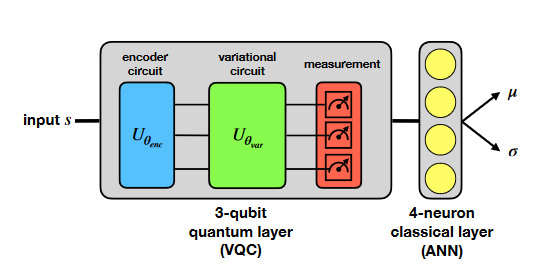
\includegraphics[width=0.6\linewidth]{img/qsac}
	\caption{Hybirid actor policy architecture, image taken from \cite{https://doi.org/10.48550/arxiv.2112.11921}}
	\label{fig:qsac}
\end{figure}\\
So of the 5 component present on this algorithm only one uses the \acrshort{vqa} with \acrshort{nn}, this can be a limitation and afterword the results using an algorithm for which every component applies it. All the test showed, are the ones with an environment that uses 2 links, this is due to a lack of time and resources. 
\subsubsection{Results with hybrid actor}
Using the previous ansatz and algorithm it was decide to apply the hybrid architecture only on the actor component applying 4 and 5 layers giving a total of respectively 100 and 112 parameters.
To confront it with a \acrshort{nn} two test were carried out using 149 and 164 parameters leading to this interesting plot. The runs could not be repeated for the lack of time and resources required, in fact the hybrid architecture took almost 19 hours to reach this point. Even if the classical one took only 4, in order to benchmark them it would require at least 1 week and as it will be noticed this kind of solution is not optimal as it will be later noticed.
One of the reasons for which this runs weren't repeated multiple times is the time and resources required, in  fact using multiple cpu or applying in the future on a gpu may reduce significantly this time. Unfortunately on the time of writing this is not possible, but it may be applied in the future.\\
Confronting result obtained using hybrid and classical components gives:  
\begin{figure}[H]
	\centering
	\includegraphics[width=0.8\linewidth]{"img/VQA and classic actor"}
	\caption{Moving average with time window of 30 with mean and standard deviation of the trend.}
	\label{fig:vqa-and-classic-actor}
\end{figure}
From this an interesting fact can be noticed: all of the test have more or less the same trend and reach the same return at around 150000 steps. As can be seen the hybrid algorithm present an higher steep curve confronting to the classical ones and is able to reach the plateau slightly faster, but there isn't a clear qurnum advantage due to the similar number of parameters and time step taken.
This is quite suspicious and could mean that the critical component may nit be the acto, but the critic. To confirm this suspect notice the plot of only the actor component that use \acrlong{nn}:
\begin{figure}[H]
	\centering
	\includegraphics[width=0.8\linewidth]{"img/classics actor"}
	\caption{Plot of the runs that uses neural netowrks for all the components.}
	\label{fig:classics-actor}
\end{figure}
As it can be noticed an increase on the number of parameters doesn't determine a great variation, instead if a plot using the hybrid algorithm and confronting them by resusing the same architecture a plot is obtained:
\begin{figure}[H]
	\centering
	\includegraphics[width=0.8\linewidth]{"img/VQA critic reduced"}
	\caption{Plot confronting vqa with reduced parameters of critic and previous ones.}
	\label{fig:vqa-critic-reduced}
\end{figure}
\vspace{0.5cm}
So effectively the most impacting component on the ability of reaching the goal of this algorithm is not the actor, but are the critic ones! Here can be found the table containing information on the structure of components where it can be noticed that except the number of params the test runs uses almost everywhere the same exact hyperparmeters:
\newline
\vspace{0.2cm}
\newline
\begin{tabular}{|c|c|c|}
	\hline
	Hyperparameters & VQA 4 layers & VQA 5 layers  \\
	\hline
	$\gamma$ & 0.99 & 0.99  \\
	\hline
	$\alpha$ & 0.2 & 0.2  \\
	\hline
	learning rate & 0.0003 & 0.0003  \\
	\hline
	memory size & 1000000 & 1000000   \\
	\hline
	optimizer & Adam & Adam  \\
	\hline
	actor neurons  & (6, VQA, (1,1)) & (6, VQA, (1,1))  \\
	\hline
	actor act. func. & (linear,relu,linear) & (linear,relu,linear) \\
	\hline
	actor params & 100 & 112 \\
	\hline
	critic neurons & (8,64,64,1) & (8,64,64,1)  \\
	\hline
	critic act. func. & (linear,relu,relu,linear) & (linear,relu,relu,linear) \\
	\hline
	critic params & 4608 & 4608 \\
	\hline
	total params & 18532 & 18544 \\
	\hline
\end{tabular}
\newline
\vspace{0.5 cm}
\newline\begin{tabular}{|c|c|c|}
	\hline
	Hyperparameters & VQA 4 layers reduced & VQA 5 layers reduced  \\
	\hline
	$\gamma$ & 0.99 & 0.99   \\
	\hline
	$\alpha$ & 0.2 & 0.2   \\
	\hline
	learning rate & 0.0003 & 0.0003   \\
	\hline
	memory size & 1000000 & 1000000   \\
	\hline
	optimizer & Adam & Adam  \\
	\hline
	actor neurons  & (6, VQA, (1,1)) & (6, VQA, (1,1))  \\
	\hline
	actor act. func. & (linear,relu,linear) & (linear,relu,linear) \\
	\hline
	actor params & 100 & 112  \\
	\hline
	critic neurons & (8,16,16,1) & (8,16,16,1)  \\
	\hline
	critic act. func. & (linear,relu,relu,linear) & (linear,relu,relu,linear) \\
	\hline
	critic params & 384 & 384\\
	\hline
	total params & 1636 & 1648\\
	\hline
\end{tabular}
\newline
\vspace{0.5 cm}
\newline
\begin{tabular}{|c|c|c|}
\hline
Hyperparameters & Actor NN 149 & Actor NN 164 \\
\hline
$\gamma$  & 0.99 & 0.99 \\
\hline
$\alpha$ & 0.2 & 0.2 \\
\hline
learning rate  & 0.0003 & 0.0003 \\
\hline
memory size  & 1000000 & 1000000 \\
\hline
optimizer  & Adam & Adam \\
\hline
actor neurons & (6,24,(1,1)) & (6,26,(1,1)) \\
\hline
actor act. func. & (linear,relu,linear) & (linear,relu,linear) \\
\hline
actor params & 149 & 164 \\
\hline
critic neurons & (8,64,64,1) & (8,64,64,1) \\
\hline
critic act. func. & (linear,relu,relu,linear) & (linear,relu,relu,linear) \\
\hline
critic params & 4608 & 4608 \\
\hline
total params  & 18581 & 18596 \\
\hline
\end{tabular}\\
\\
The reason for which the toal parameters is so high links to the fact that there are 4 critic components that are required in order for the algorithm to work and learn.
\subsubsection{Results with hybrid actor and critic}
Now that the previous test have demonstrated that critic is the component that determines the most on performace the following test will use the hybrid algorithm used for the actor and apply it on critic. During the first tests we noticed that the previous structure used for actor, isn't good for the critic due to maybe a high non-linearity of the map required. For this reason the previous structure was modifided by adding a hidden layer before the output to increase the expressivity of non-linearity. This is the schematic:
\begin{figure}[!h]
	\centering
	\resizebox {1.0\linewidth} {!} {
	\begin{tikzpicture}
		\node[draw, label = {repeat $n$ times}](vqc) {
			\begin{quantikz}
				\qw & \gate[style={fill=red!70}]{R_x(\lambda x)} & 	\gate[style={fill=cyan}]{R_y(\theta)}& \gate[style={fill=cyan}]{R_z(\theta)} & \ctrl{1} & \qw & \qw & \qw & \qw & \targ{} & \qw \\
				\qw & \gate[style={fill=red!70}]{R_x(\lambda x)} & 	\gate[style={fill=cyan}]{R_y(\theta)}& \gate[style={fill=cyan}]{R_z(\theta)} & \targ{} & \ctrl{1} & \qw & \qw & \qw & \qw & \qw \\
				\qw & \gate[style={fill=red!70}]{R_x(\lambda x)} & 	\gate[style={fill=cyan}]{R_y(\theta)}& \gate[style={fill=cyan}]{R_z(\theta)} & \qw & \targ{} & \ctrl{1} & \qw & \qw & \qw & \qw \\
				\qw & \gate[style={fill=red!70}]{R_x(\lambda x)} & 	\gate[style={fill=cyan}]{R_y(\theta)}& \gate[style={fill=cyan}]{R_z(\theta)} & \qw & \qw & \targ{} & \ctrl{1} & \qw & \qw & \qw \\
				\qw & \gate[style={fill=red!70}]{R_x(\lambda x)} & 	\gate[style={fill=cyan}]{R_y(\theta)}& \gate[style={fill=cyan}]{R_z(\theta)} & \qw & \qw & \qw & \targ{} & \ctrl{1} & \qw & \qw \\
				\qw & \gate[style={fill=red!70}]{R_x(\lambda x)} & 	\gate[style={fill=cyan}]{R_y(\theta)}& \gate[style={fill=cyan}]{R_z(\theta)} & \qw & \qw & \qw & \qw & \targ{} & \ctrl{-5} & \qw \\
			\end{quantikz}
		};
		\node[right = -4mm of vqc, label = {measure}](measure) {
			\begin{quantikz}
				\qw & \meter{} & \qw \\
				\qw & \meter{} & \qw \\
				\qw & \meter{} & \qw \\
				\qw & \meter{} & \qw \\
				\qw & \meter{} & \qw \\
				\qw & \meter{} & \qw \\
			\end{quantikz}
		};
		\node[circle, above left = -6.5mm and 10mm of vqc , fill=orange, label={input}] (I1) {};
		\node[circle, below = 8mm of I1 , fill=orange] (I2) {};
		\node[circle, below = 8mm of I2 , fill=orange] (I3) {};
		\node[circle, below = 8mm of I3 , fill=orange] (I4) {};
		\node[circle, below = 8mm of I4 , fill=orange] (I5) {};
		\node[circle, below = 8mm of I5 , fill=orange] (I6) {};
		\foreach \i in {1,2,3,4,5,6}{
			\path (I\i) edge (-5.85,3.35);
			\path (I\i) edge (-5.85,2.15);
			\path (I\i) edge (-5.85,0.95);
			\path (I\i) edge (-5.85,-0.35);
			\path (I\i) edge (-5.85,-1.55);
			\path (I\i) edge (-5.85,-2.75);
		}
		\node[circle, above right = -6.8mm and 8mm of measure , fill=orange, label={hidden}] (H1) {};
		\node[circle, below = 8mm of H1 , fill=orange] (H2) {};
		\node[circle, below = 8mm of H2 , fill=orange] (H3) {};
		\node[circle, below = 8mm of H3 , fill=orange] (H4) {};
		\node[circle, below = 8mm of H4 , fill=orange] (H5) {};
		\node[circle, below = 8mm of H5 , fill=orange] (H6) {};
		\foreach \i in {1,...,6}{
			\path (H\i) edge (7.7,3.35);
			\path (H\i) edge (7.7,2.15);
			\path (H\i) edge (7.7,0.95);
			\path (H\i) edge (7.7,-0.35);
			\path (H\i) edge (7.7,-1.55);
			\path (H\i) edge (7.7,-2.8);
		}
		\node[circle, below right = 15mm and 15mm of H2, fill=orange, label={output}] (O1) {};
		\foreach \i in {1,...,6}{
			\path (H\i) edge (O1);
		}
	\end{tikzpicture}	
	}
	\caption{Structure for critic hybrid}
	\label{critic hybrid}
\end{figure}\\
As it can be seen from the plot \ref{fig:fully_vs_partial_quantum} by converting all components to hybrid architecture it was able to have a performance veery similar to the ones with only hybrid actor. As it will be seen later this means that a smaller component that uses few parameters is able to reach the same performance of one with more on the Neural network. Reason for which this line is interrupted after only 250000 steps is maily due to the high time required, in fact to reach that step the fully hybrid algorithm took more than a week and after concluding that the algorithm was performing very similarly to the actor hybrid it was stopped.\\
\begin{figure}[H]
	\centering
	\includegraphics[width=1.0\linewidth]{"img/fully_vs_partial_quantum"}
	\caption{Comparision between only actor hybrid and all components hybrid.}
	\label{fig:fully_vs_partial_quantum}
\end{figure}
Afterward to have a detailed cased for which multiple configuration with different size of the neural network were conducted in order to understand what kind of advantage was expected to confront the run of all-hybrid components and all neural networks. As it can be noticed from \ref{fig:all-classical-results} increasing the size of \acrlong{nn} and keeping the actor equal for all runs doesn't mean that there is an increase on performance and unfortunately the run that uses the least number of neurons is not able to reach the objective to have a score at least -40 as average. The choice on using 21 neurons is not casual, but it has been decided in order to have a similar number of parameters equal to the run that uses all hybrid components.
\begin{figure}[H]
	\centering
	\includegraphics[width=0.9\linewidth]{"img/All classical results"}
	\caption{All classical runs with an actor component of 149 parameters}
	\label{fig:all-classical-results}
\end{figure}
\begin{figure}[H]
	\centering
	\includegraphics[width=0.9\linewidth]{"img/Best classical vs all hybrid results"}
	\caption{Plot of best classical runs and all-hybrid}
	\label{fig:best-classical-vs-all-hybrid-results}
\end{figure}
\newpage

So by looking at \ref{fig:best-classical-vs-all-hybrid-results} an important result can be obtained, the all-hybrid run is able to reach a similar performance of all neural networks components that use an higher number of neurons to reach the objective with a similar trend and time steps required. \textbf{But if the neural network model uses a similar parameter number of all-hybrid model then it will not be able to reach the objective}.

